\documentclass[a4paper,11pt]{exam}
\printanswers % pour imprimer les réponses (corrigé)
%\noprintanswers % Pour ne pas imprimer les réponses (énoncé)
\addpoints % Pour compter les points
% \noaddpoints % pour ne pas compter les points
%\qformat{\textbf{\thequestion ) } }
%\qformat{\textbf{\thequestion )} (\thepoints) \\} % Pour définir le style des questions (facultatif)
\usepackage{color} % définit une nouvelle couleur
\shadedsolutions % définit le style des réponses
% \framedsolutions % définit le style des réponses
\definecolor{SolutionColor}{rgb}{0.8,0.9,1} % bleu ciel
\renewcommand{\solutiontitle}{\noindent\textbf{Solution:}\par\noindent} % Définit le titre des solutions




\makeatletter

\def\maketitle{{\centering%
	\par{\huge\textbf{\@title}}%
	\par{\@date}%
	\par}}

\makeatother

\lhead{NOM Pr\'enom :}
\rhead{\textbf{Les r\'eponses doivent \^etre justifi\'ees}}
\cfoot{\thepage / \pageref{LastPage}}


%\usepackage{../../pas-math}
%\usepackage{../../moncours}


%\usepackage{pas-cours}
%-------------------------------------------------------------------------------
%          -Packages nécessaires pour écrire en Français et en UTF8-
%-------------------------------------------------------------------------------
\usepackage[utf8]{inputenc}
\usepackage[frenchb]{babel}
\usepackage[T1]{fontenc}
\usepackage{lmodern}
\usepackage{textcomp}



%-------------------------------------------------------------------------------

%-------------------------------------------------------------------------------
%                          -Outils de mise en forme-
%-------------------------------------------------------------------------------
\usepackage{hyperref}
\hypersetup{pdfstartview=XYZ}
%\usepackage{enumerate}
\usepackage{graphicx}
\usepackage{multicol}
\usepackage{tabularx}
\usepackage{multirow}


\usepackage{anysize} %%pour pouvoir mettre les marges qu'on veut
%\marginsize{2.5cm}{2.5cm}{2.5cm}{2.5cm}

\usepackage{indentfirst} %%pour que les premier paragraphes soient aussi indentés
\usepackage{verbatim}
\usepackage{enumitem}
\usepackage[usenames,dvipsnames,svgnames,table]{xcolor}

\usepackage{variations}

%-------------------------------------------------------------------------------


%-------------------------------------------------------------------------------
%                  -Nécessaires pour écrire des mathématiques-
%-------------------------------------------------------------------------------
\usepackage{amsfonts}
\usepackage{amssymb}
\usepackage{amsmath}
\usepackage{amsthm}
\usepackage{tikz}
\usepackage{xlop}
%-------------------------------------------------------------------------------



%-------------------------------------------------------------------------------


%-------------------------------------------------------------------------------
%                    - Mise en forme avancée
%-------------------------------------------------------------------------------

\usepackage{ifthen}
\usepackage{ifmtarg}


\newcommand{\ifTrue}[2]{\ifthenelse{\equal{#1}{true}}{#2}{$\qquad \qquad$}}

%-------------------------------------------------------------------------------

%-------------------------------------------------------------------------------
%                     -Mise en forme d'exercices-
%-------------------------------------------------------------------------------
%\newtheoremstyle{exostyle}
%{\topsep}% espace avant
%{\topsep}% espace apres
%{}% Police utilisee par le style de thm
%{}% Indentation (vide = aucune, \parindent = indentation paragraphe)
%{\bfseries}% Police du titre de thm
%{.}% Signe de ponctuation apres le titre du thm
%{ }% Espace apres le titre du thm (\newline = linebreak)
%{\thmname{#1}\thmnumber{ #2}\thmnote{. \normalfont{\textit{#3}}}}% composants du titre du thm : \thmname = nom du thm, \thmnumber = numéro du thm, \thmnote = sous-titre du thm

%\theoremstyle{exostyle}
%\newtheorem{exercice}{Exercice}
%
%\newenvironment{questions}{
%\begin{enumerate}[\hspace{12pt}\bfseries\itshape a.]}{\end{enumerate}
%} %mettre un 1 à la place du a si on veut des numéros au lieu de lettres pour les questions 
%-------------------------------------------------------------------------------

%-------------------------------------------------------------------------------
%                    - Mise en forme de tableaux -
%-------------------------------------------------------------------------------

\renewcommand{\arraystretch}{1.7}

\setlength{\tabcolsep}{1.2cm}

%-------------------------------------------------------------------------------



%-------------------------------------------------------------------------------
%                    - Racourcis d'écriture -
%-------------------------------------------------------------------------------

% Angles orientés (couples de vecteurs)
\newcommand{\aopp}[2]{(\vec{#1}, \vec{#2})} %Les deuc vecteurs sont positifs
\newcommand{\aopn}[2]{(\vec{#1}, -\vec{#2})} %Le second vecteur est négatif
\newcommand{\aonp}[2]{(-\vec{#1}, \vec{#2})} %Le premier vecteur est négatif
\newcommand{\aonn}[2]{(-\vec{#1}, -\vec{#2})} %Les deux vecteurs sont négatifs

%Ensembles mathématiques
\newcommand{\naturels}{\mathbb{N}} %Nombres naturels
\newcommand{\relatifs}{\mathbb{Z}} %Nombres relatifs
\newcommand{\rationnels}{\mathbb{Q}} %Nombres rationnels
\newcommand{\reels}{\mathbb{R}} %Nombres réels
\newcommand{\complexes}{\mathbb{C}} %Nombres complexes


%Intégration des parenthèses aux cosinus
\newcommand{\cosP}[1]{\cos\left(#1\right)}
\newcommand{\sinP}[1]{\sin\left(#1\right)}


%Probas stats
\newcommand{\stat}{statistique}
\newcommand{\stats}{statistiques}
%-------------------------------------------------------------------------------

%-------------------------------------------------------------------------------
%                    - Mise en page -
%-------------------------------------------------------------------------------

\newcommand{\twoCol}[1]{\begin{multicols}{2}#1\end{multicols}}


\setenumerate[1]{font=\bfseries,label=\textit{\alph*})}
\setenumerate[2]{font=\bfseries,label=\arabic*)}


%-------------------------------------------------------------------------------
%                    - Elements cours -
%-------------------------------------------------------------------------------





%\usepackage{fullpage}
\author{\ }
\date{05 Février 2020}
\title{$6^e C$ : DS num\'ero 4}


\begin{document}
%	\usepackage{fancyhdr}
%	
%	\pagestyle{fancy}
%	\fancyhf{}
	%\rhead{Share\LaTeX}

	\maketitle
	
\begin{center}
	\textbf{Calculatrice interdite, le soin et la qualité de la rédaction seront pris en compte}
\end{center}

\begin{small}
	\begin{center}
		\begin{tabular}{|@{\ }l@{\ }|@{\ }c@{\ }|@{\ }c@{\ }|@{\ }c@{\ }|@{\ }c@{\ }|}
			\hline
			\textbf{Compétence} & \textbf{MI} & \textbf{MF} & \textbf{MS} & \textbf{TBM} \\
			\hline
			\textbf{Représenter} (Reconnaître et utiliser des premiers éléments de codage d'une figure. ) &  \ \ & \ \ & \ \ & \ \  \\
			\hline	
			\textbf{Raisonner} (Raisonner à l'aide de propriétés de figures.) & \ \ & \ \ &  \ \  & \ \ \\
			\hline
			%			 \textbf{Communiquer} (Expliquer sa démarche, son raisonnement ) &  \ \ & \ \ & \ \ & \ \  \\
			%			\hline
		\end{tabular}
	\end{center}
\end{small}	

	
	
	

%\newpage

\section{Placer des points (2 points)}

\begin{questions}
	\question[1] Reproduire une figure semblable à celle ci dessous. Les dimensions n'ont pas d'importance.
	
	

	\question[2] Placer les points $B$, $C$, $D$ et $E$ %\textbf{sur cette figure}
	, sachant que :
	
	\begin{multicols}{2}
		
		\begin{center}
			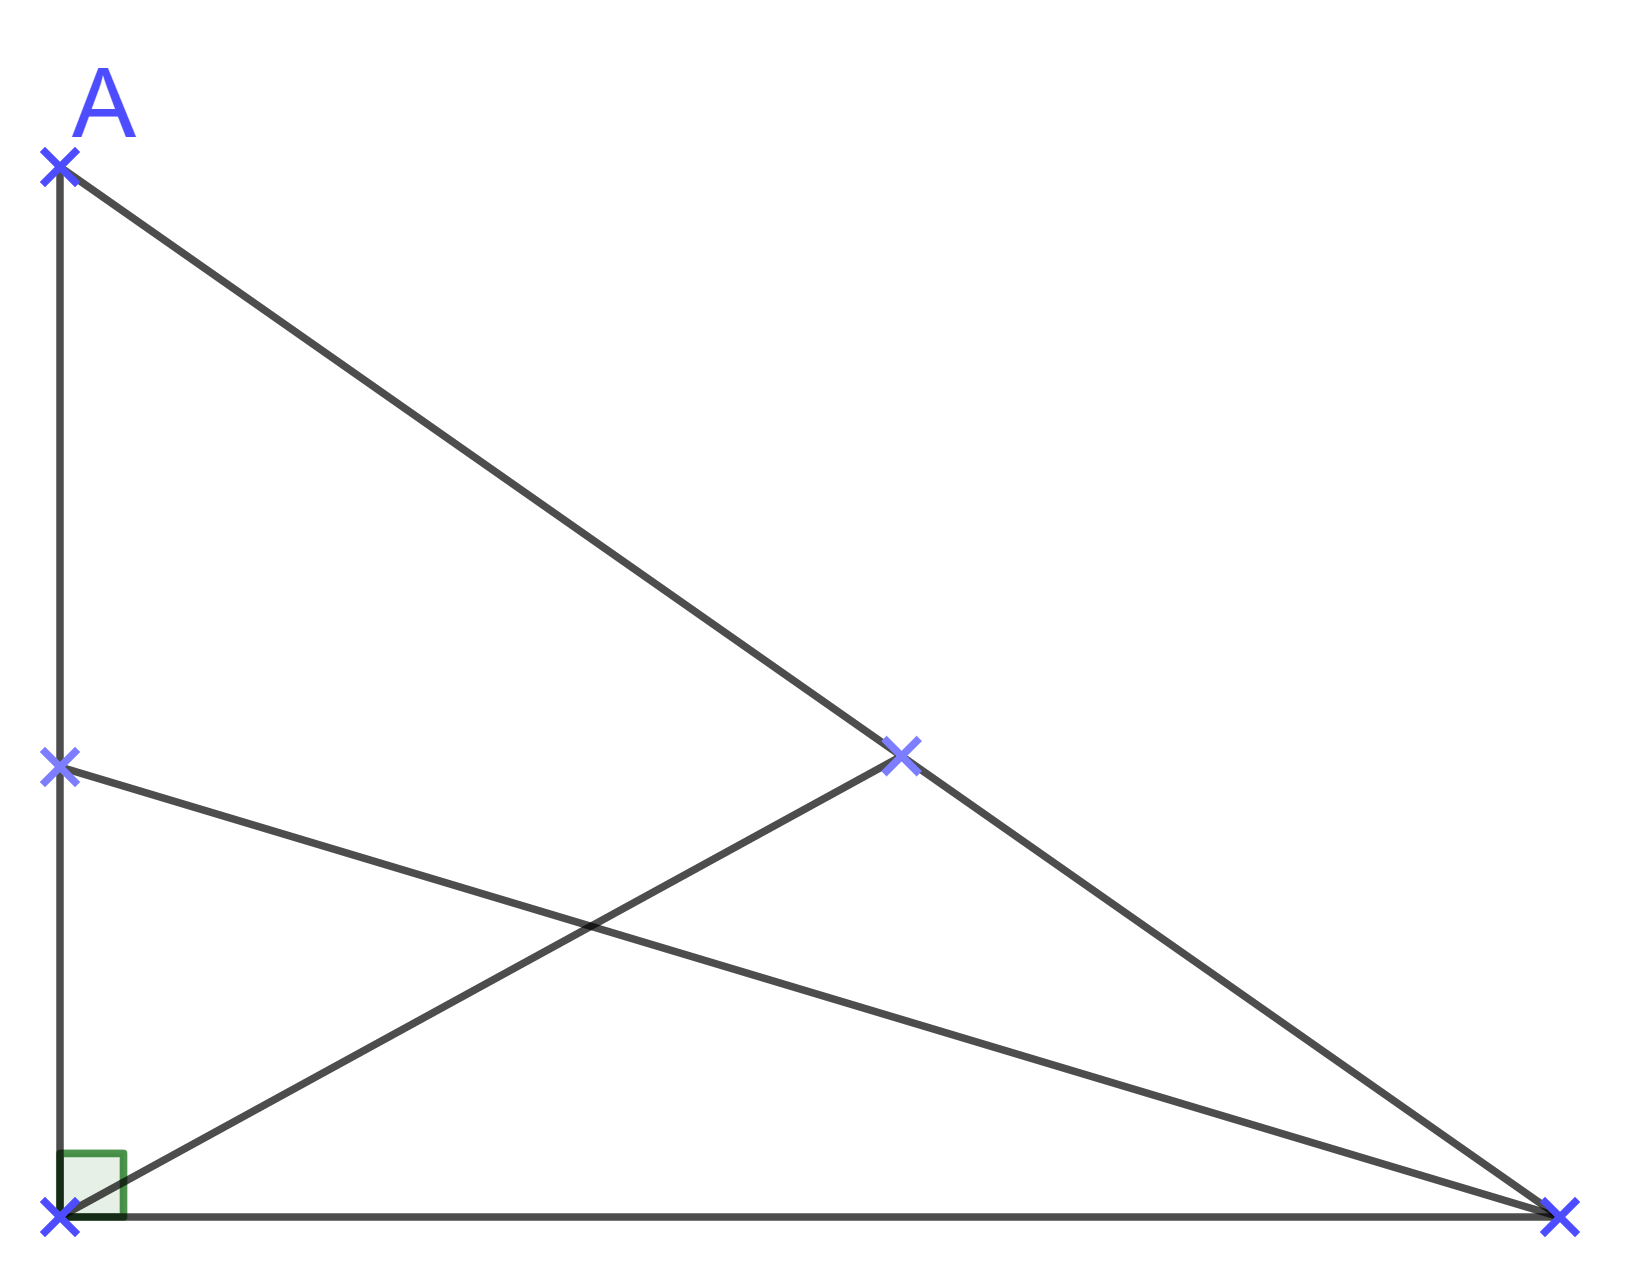
\includegraphics[scale=0.15]{img/ex1}
		\end{center}
		
		\begin{itemize}
			\item $\widehat{ABC}$ est droit;
			\item $\widehat{BDC}$ est aigu;
			\item $\widehat{CEB}$ est obtus;
		\end{itemize}
	\end{multicols}
	
	
\end{questions}




\section{Classer des angles (4 points)}

\begin{questions}
	\question[4] Pour chaque angle ci-dessous, remplir \textbf{sur cette feuille  }le tableau suivant avec ses différentes caractéristiques.
	
	 \begin{center}
	 	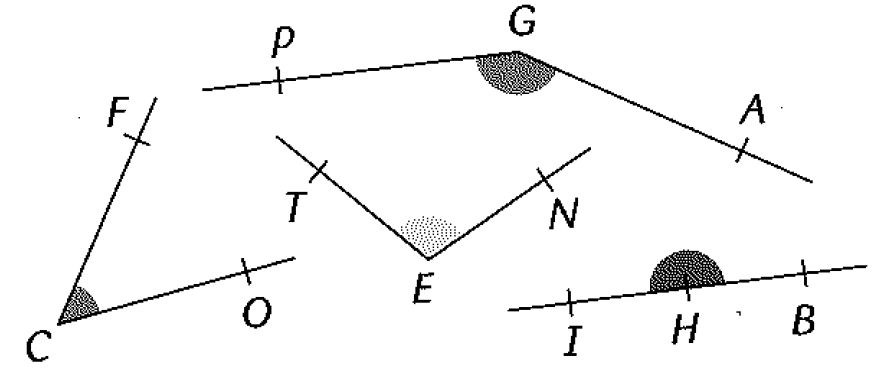
\includegraphics[scale=0.4]{img/angles}
	 \end{center}

\begin{tabular}{|c|c|c|c|}
	\hline
	\textbf{Angle} & \textbf{Sommet} & \textbf{Côtés} & \textbf{Type} \\ \hline
	&                 &                &               \\ \hline
	&                 &                &               \\ \hline
	&                 &                &               \\ \hline
	&                 &                &               \\ \hline
	%&                 &                &               \\ \hline
\end{tabular}

\end{questions}



\begin{mydef}
	\begin{itemize}
		\iftoggle{eleve}{%
			\item \hrulefill
			\item \hrulefill
		}{%
			\item Un angle se mesure en \kw{degrés ($\degree$)};
			\item On utilise un \kw{rapporteur}.
		}
		
		
	\end{itemize}
\end{mydef}

\begin{myexs}
	\begin{itemize}
		
		\iftoggle{eleve}{%
			\item Un angle nul mesure 
			\item Un angle aigu mesure 
			\item Un angle droit mesure 
			\item Un angle obtus mesure 
			\item Un angle plat mesure 
			\item Un cercle mesure 
		}{%
			\item Un angle nul mesure 0\degree;
			\item Un angle aigu mesure entre 0 et 90\degree;
			\item Un angle droit mesure 90\degree;
			\item Un angle obtus mesure entre 90 et 180\degree;
			\item Un angle plat mesure 180\degree.
			\item Un cercle mesure 360\degree.
		}
		
	\end{itemize}
\end{myexs}

\section{Construction (6 points)}

\begin{questions}
	\question[3] Construire en vraie grandeur la figure ci-dessous.
	\begin{center}
		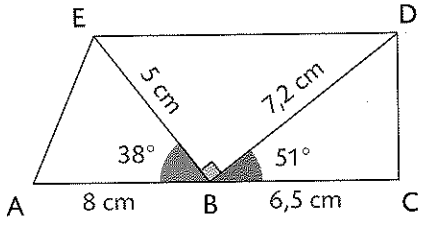
\includegraphics[scale=0.7]{img/figure}
	\end{center}

	\question 
		\begin{parts}
			\part[1] Sur votre figure, les points A, B et C semblent-t-ils alignés.
			
			\part[2] Le sont-ils vraiment ? Justifier votre réponse.
		\end{parts}
\end{questions}

\section{Repérage (4 points)}

Dans la grille ci-dessous :

\begin{multicols}{2}
	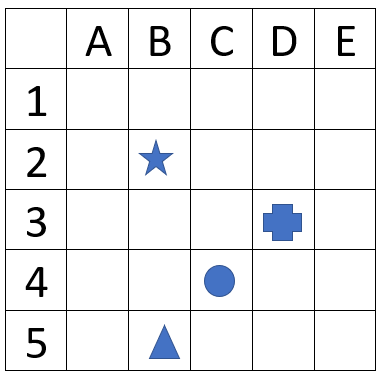
\includegraphics[scale=0.5]{img/grille}
	
	\begin{questions}
		\question[1] Donner les coordonnées de chaque symbole.
		
		\question[1\half] Placer en bleu \textbf{dans cette grille} la nouvelle position du triangle après les mouvements suivants :  {\Large $\Rightarrow \; \Rightarrow \; \Uparrow  \; \Uparrow \; \Leftarrow$}.
		
		\question[1\half] Quels mouvement devrait-il faire \textbf{depuis sa nouvelle position} pour arriver en $A2$.
	\end{questions}
\end{multicols}




\section*{Bonus : Ballon de football (3 points)}
Un ballon de football est composé de 32 pièces qui sont des hexagones et des pentagones.

\begin{questions}
	\question[3] Reproduire la figure ci-dessous en prenant 4cm pour la longueur des cotés des polygones.
\end{questions}

\begin{multicols}{2}
	\begin{center}
		
\includegraphics[scale=0.4]{img/foot1}
	\end{center}

	\begin{center}
		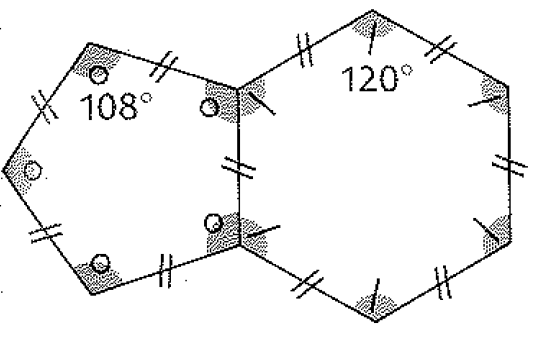
\includegraphics[scale=0.55]{img/foot2}
	\end{center}
\end{multicols}

\label{LastPage}

\end{document}